%todo : THUSC2016 CF848D CF750G
\documentclass{beamer}
\usetheme[navigation]{UMONS}
\usepackage{ctex}
\usepackage[english]{babel}
\usepackage{amsmath}
\usepackage{graphicx}

\title[动态规划:思维与优化]{动态规划:思维与优化}
\author[Simphoni]{Simphoni}
\begin{document}
\maketitle
\section{Overview}
\begin{frame}
  \frametitle{Overview}
  \centering
  \tableofcontents
\end{frame}

\section{The art of DP}

\subsection{Ebola}
\begin{frame}
  \frametitle{ASC46 Ebola}
  \begin{block}{Statement}
    \setlength{\parindent}{2em}
    有$n\ (n\le 4000)$个村庄按顺序依次排列在一条直线上,第$i$个村庄有
    $a_i\ (a_i\le 10^9)$个人患病,每天傍晚第$i$个村庄中的患者将病毒传染给\alert{另
      外}$a_i$个人,然后这原来的$a_i$个患者病逝,假设每个村庄的人足够
    多。
    
    你现在要从$1$号村庄出发,终止这次的疫情并最终到达$n$号点,每天你可以做下列一件事:
    \begin{itemize}
    \item 移动到一个相邻的村庄
    \item 救治你所在的村庄的患者(则该村庄从当天开始无人病逝)
    \end{itemize}
    由于一些原因,如果某一步你选择向$1$号村庄移动,你就必须按
    照标号从大到小访问你\alert{曾经经过,但是没有救治过}的村庄并依次
    救治。
    
    要求最小化病逝的人数。
  \end{block}
\end{frame}

\begin{frame}
  \frametitle{ASC46 Ebola}
  \begin{block}{Hint}
    \begin{itemize}
    \item 可以将村庄分成若干段,每段经过$1$或$3$次 \pause
    \item 对于每个区间$[L,R]$,分别求出经过$1$和$3$次的最小代价 \pause
    \item 最后一次DP合成整个区间即可,时间复杂度$O(n^2)$
    \end{itemize}
  \end{block}
\end{frame}

\subsection{Elegent}
\begin{frame}
  \frametitle{ASC45 Elegent}
  \begin{block}{Statement}
    \setlength{\parindent}{2em}
    你有一行$1,2,\cdots,2^n\ (n\le 12)$的数,每次你可以将序列对半分开,并且选择是否将左右两半交换位置。然后对两边的序列递归操作,直到长度为1。\\
    给定常数$a,b,c,m$。设最后得到的序列是$p_1,p_2,\cdots,p_{2^n}$,那么代价为$cost=\sum_{i=1}^{2^n-1}((a*p_i+b*p_{i+1}+c*(p_i\oplus p_{i+1}))\mod m)$。\\
    你要最小化$cost$。
  \end{block}
\end{frame}

\begin{frame}
  \frametitle{ASC45 Elegent}
  \begin{block}{Hint}
    \begin{itemize}
    \item $a,b,c,m$的作用仅仅是为了减小读入量 \pause
    \item 相当于一棵满二叉树,允许任意交换每个节点的左右子树 \pause
      \vspace{0.7em}
    \item 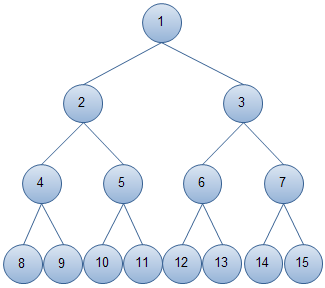
\includegraphics[width=0.4\textwidth]{full.png}
    \end{itemize}
  \end{block}
\end{frame}

\begin{frame}
  \frametitle{ASC45 Elegent}
  \begin{block}{Hint}
    \begin{itemize}
    \item 由于允许交换的性质,所有节点都是等价的 \pause
    \item 只要考虑一个符合要求的排列具有的性质即可 \pause
    \item 观察到对于序列中特定位置的数,只要每次走到特定深度的父节点的另一棵子树中就能保证是满足要求的排列 \pause
    \item 令$dp_{i,j}$表示确定了$i$个数,最后一个是$j$的最小代价 \pause
    \item 枚举下一步能到达的节点,复杂度$O(n*2^{2n})$
    \end{itemize}
  \end{block}
\end{frame}

\subsection{Shake It!}
\begin{frame}
  \frametitle{Codeforces 848D Shake It!}
  \begin{block}{Statement}
    \setlength{\parindent}{2em}
    一张图一开始有两个点$s,t$,以及无向边$(s,t)$。你要进行$n\ (n\le 50)$次操作,每次操作选择一条边$(u,v)$,并新建一个点$k$,加入无向边$(u,k)$和$(k,v)$。\\
    求最终能够得到的图中有几张最大流为$m$。同构的图只计算一次。\\
    图$G_1$和$G_2$同构当且仅当:
    \begin{itemize}
    \item 存在一个排列$p_1,p_2,\cdots,p_{n+2}$,使得$\forall (u,v)\in E(G_1)\ \exists (p_u,p_v)\in E(G_2)$
    \item $p_s=s$且$p_t=t$
    \end{itemize}
  \end{block}
\end{frame}


\begin{frame}
  \frametitle{Codeforces 848D Shake It!}
  \begin{block}{Hint}
    \begin{itemize}
    \item 同构的限制等价于“基于同一条边的子图之间是无序的” \pause
    \item 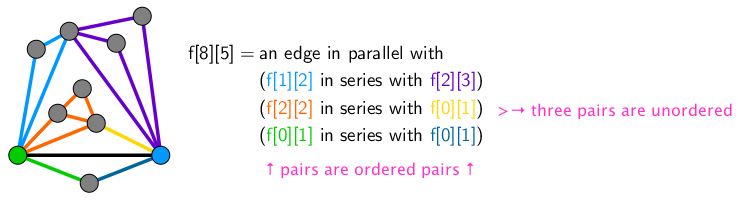
\includegraphics[width=0.85\textwidth]{flow.png}
    \end{itemize}
  \end{block}
\end{frame}

\begin{frame}
  \frametitle{Codeforces 848D Shake It!}
  \begin{block}{Hint}
    \begin{itemize}
    \item 考虑$f_{i,j}$表示操作$i$次得到的图最小割为$j$的图的计数 \pause
    \item 那么若有$c$个这样的图基于同一条边,则仅考虑这$c$张图时的方案数为$\binom{f_{i,j}+c-1}{c-1}$ \pause
    \item 用背包的方式加入,对每一对$i,j$枚举$c$ \pause
    \item $g_{a+c*i,b+c*j} \leftarrow g_{a,b}*\binom{h_{i,j}+c-1}{c-1}$
    \item $h_{a+c+1,\min(b,d)+1}\leftarrow f_{a,b}*f_{c,d}$
    \item $f_{i,j}\leftarrow g_{i,j}$\pause
    \item 由于$H(n)\le n\log n$,故复杂度为$O(n^4\log n)$
    \end{itemize}    
  \end{block}
\end{frame}

\section{Linear Recurrence}
\subsection{from NOIP to NOI}

\begin{frame}
  \frametitle{The problem of Linear Recurrence}
\end{frame}

\end{document}
